% !TEX TS-program = pdflatex
\documentclass[11pt, letterpaper]{article}

%% Packages
\usepackage[utf8]{inputenc}
\usepackage[margin=1in]{geometry}
\usepackage{setspace}
\usepackage{hyperref}
\usepackage{parskip}
\usepackage{mathtools}
\usepackage{amssymb}
\usepackage{mathrsfs}
\usepackage[figurewithin=section]{caption}
\usepackage{float}
\usepackage[style=ieee, sorting=none]{biblatex}

%% Document Setup
\pagestyle{plain}
\onehalfspacing
\numberwithin{equation}{section}
\addbibresource{ref.bib}
\begin{document}

%% First Page
\title{Review of Noise Cancellation Technology in the Acoustical Realm}
\author{Raj Patel, Andrew Trimper}
\date{November 16, 2020}
\maketitle
\tableofcontents
\newpage

%% Abstract
\section{Abstract}

Noise cancellation is the process by which noise impacting a system is nullified in order to improve system functionality. The noise cancellation technology is wide-ranging in applications, and has seen use in acoustics, radio-frequency (RF), and electronics, among other spaces. This review focuses on the application of noise cancellation in the acoustical realm. The topic is first introduced broadly to give scope to the importance of noise cancellation as it applies to acoustics. Acoustical noise cancellation is then broken down into two variants: passive noise cancellation (PNC) and active noise cancellation (ANC). ANC is studied significantly in this review which reflects the distribution of state-of-the-art literature across these two variants. Fourier analysis is presented as a tool used to enable certain ANC methods. A more popular adaptive ANC algorithm, Filtered-x Least Mean Square (FXLMS), is examined in detail to provide a glimpse of advances in acoustical noise cancellation. Finally, the applications of noise cancellation are discussed. The goals of this review are to provide a background and delineate the role of Fourier analysis in acoustical noise cancellation. The interplay between Fourier analysis and acoustical noise cancellation is essential, as a lot of advances in the field of acoustical noise cancellation have come as its direct result.
\\
\textbf{Keywords}: Acoustics, Active Noise Cancellation, Adaptive Filter, Digital Signal Processing (DSP), Feedforward Control, Fourier Analysis, Passive Noise Cancellation

%% Introduction
\section{Introduction}

Acoustical noise cancellation is commonly used in many aspects of modern society, and plays a versatile role in the everyday quality of life for a variety of individuals. Although the public perception of this technology is limited primarily to noise-cancelling headphones, acoustical noise cancellation exists in a wide range of applications such as cars, planes, and ventilation ducts \cite{kuo}. For cars, PNC is utilized to reduce the wind noise and tire noise from the perspective of the driver and passengers. ANC is sometimes used in higher-end vehicles when more resources can be allocated to reducing noise \cite{chen}. In planes, both PNC and ANC are used extensively. The external noise from jet engines and passing wind is intense, and would cause hearing damage to plane occupants if not accounted for by design \cite{roy}. These issues and applications of acoustical noise cancellation exemplify the role and importance of Fourier analysis in emerging technologies, and so necessitates a literature review on the topic.

Section \ref{sec:PNC} contains a brief overview and methodology of PNC. Section \ref{sec:ANC_Basics} covers critical details necessary to grasp how ANC differs from PNC, and how ANC is designed and developed. Section \ref{sec:ANC_FXLMS} dives further into ANC by looking at the FXLMS algorithm and its use of adaptive filtering.

%% Passive Noise Cancellation
\section{Passive Noise Cancellation}
\label{sec:PNC}

PNC methods use physical impedance or absorption as a means of reducing unwanted noise without applying external energy to the system. PNC uses materials that excite at similar frequencies as the resident noise waves, and result in friction energy losses that dissipate said noise waves \cite{lu}. PNC can block a wide range of frequencies by, for example, covering ear canals, or intentionally placing panels at key points of walls in a given room.

PNC can be a useful and cost-effective solution for reducing high-frequency noise; however, PNC increases in size and cost when designed to reduce lower frequencies \cite{kuo}. In this regard, ANC is a size and cost-effective alternative to PNC for reducing lower frequencies \cite{kuo}.

%% Active Noise Cancellation Basics
\section{Active Noise Cancellation Basics}
\label{sec:ANC_Basics}

A discussion of an ANC solution and implementation requires the understanding of key mathematical concepts.

%% Mathematical Foundation
\subsection{Mathematical Foundation}

%% Domain Transform
\subsubsection{Domain Transform}

The Fourier transform (FT) is used to convert signals in the time-domain into signals in the frequency-domain:

\begin{equation}
    \mathcal{F}(s) = \int \limits_{-\infty}^\infty f(t) e^{-j 2 \pi t s}\ dt \text{ ,}
\end{equation}

where $s$ is the continuous frequency variable, $\mathcal{F}$ is the frequency-domain function, $t$ is the continuous time variable, and $f$ is the time-domain function.

Since noise is sampled discretely in a real-time system, the Fourier transform is altered to take into account the size of the sample set (i.e. the discrete-time Fourier transform (DFT)):

\begin{equation}
    \mathcal{F}(v) = \frac{1}{N} \sum \limits_{\tau = 0}^{N - 1} f(\tau) e^{-j 2 \pi \tau \frac{v}{N}} \text{ ,}
\end{equation}

where $v$ is the discrete frequency variable, $\mathcal{F}$ is the frequency-domain function, $N$ is the total number of samples, $\tau$ is the discrete time variable, and $f$ is the time-domain function \cite{bracewell}. The fast Fourier transform (FFT) is an algorithm that makes use of the DFT \cite{bracewell}.

\pagebreak

The inverse discrete-time Fourier transform (IDFT) is used to convert discrete frequency-domain data back into discrete real-time data for a real-time system \cite{bracewell}:

\begin{equation}
    f(\tau) = \sum \limits_{v = 0}^{N - 1} \mathcal{F}(v) e^{j 2 \pi \tau \frac{v}{N}} \text{ ,}
\end{equation}

where $\tau$ is the discrete time variable, $f$ is the time-domain function, $v$ is the discrete frequency variable, $N$ is the total number of samples, and $\mathcal{F}$ is the frequency-domain function \cite{bracewell}. The inverse fast Fourier transform (IFFT) is an algorithm that makes use of the IDFT \cite{bracewell}.

%% Wave Superposition
\subsubsection{Wave Superposition}

The superposition of different propagating waves results in a new wave that is a function of the original waves \cite{roy}.

Constructive interference of waves with the same frequency results in the sum of the amplitudes of all waves at any given point. Constructive interference occurs when the phase difference between all of the waves is

\begin{equation}
    \phi_j - \phi_i = 2 \pi n \text{ ,}
\end{equation}

where $\phi_x$ is the phase angle of the wave $x$ in radians, $i \neq j$, and $n \in \mathbb{Z}$.

Destructive interference of waves with the same frequency and same amplitude results in $0$, or nullification, at any given point. Destructive interference occurs when the phase difference between all of the waves is

\begin{equation}
    \phi_j - \phi_i = \pi (2n + 1) \text{ ,}
\end{equation}

where $\phi_x$ is the phase angle of the wave $x$ in radians, $i \neq j$, and $n \in \mathbb{Z}$.

\pagebreak

%% Feedforward Control System
\subsubsection{Feedforward Control System}

A feedforward control system sends the input of the system both to the plant and directly to the summing junction. The environmental noise is the input into the system, $u(\tau)$ or $\mathcal{F}^{-1}[U(v)]$. The dynamics operating on the input is the nonlinear plant, $G(v)$. The new signal produced by the plant is another signal sent to the summing junction. The summation of the input of the system and the output of the plant is sent into the environment as the output of the system, $y(\tau)$ or $\mathcal{F}^{-1}[Y(v)]$. The generic linearized transfer function for a feedforward control system is given by

\begin{equation}
    y(\tau) = \mathcal{F}^{-1}[Y(v)] = \mathcal{F}^{-1}[u(\tau)] - G(v) \mathcal{F}^{-1}[u(\tau)] = U(v) - G(v) U(v) \text{ ,}
\end{equation}

where $\tau$ is the time-domain variable, $v$ is the frequency-domain variable, $\mathcal{F}$ is the DFT as an operator, $\mathcal{F}^{-1}$ is the IDFT as an operator, both $y(\tau) \text{ and } Y(v)$ represent the (same) output of the system, both $u(\tau) \text{ and } U(v)$ represent the (same) input of the system, and $G(v)$ is the transfer function of the system.

%% Frequency-Domain Feedforward Solution
\subsection{Frequency-Domain Feedforward Solution}

Fundamentally, ANC reduces undesired noise waves by producing an anti-noise wave that eliminates the original noise wave through destructive interference. ANC can be modeled as a feedforward control problem (Fig. \ref{fig:ANC_gen}). The environmental noise is detected by the system through a reference microphone, and is propagated forward through the channel to the error microphone. The discrete-time noise data from the reference microphone is converted to discrete frequency-domain data using the FFT. Based on the reference microphone and the error microphone, the ANC system generates new discrete frequency-domain data with the same amplitude and shifted phase \cite{kajikawa}. The new discrete frequency-domain data is converted into discrete-time data using the IFFT, and broadcasted by a speaker. The error microphone measures the new noise wave as a result of the superposition of the broadcasted signal and the original noise wave; after being converted to frequency-domain data using the FFT, the new noise wave is sent to the ANC system, as mentioned earlier.

\begin{figure}[H]
	\begin{center}
		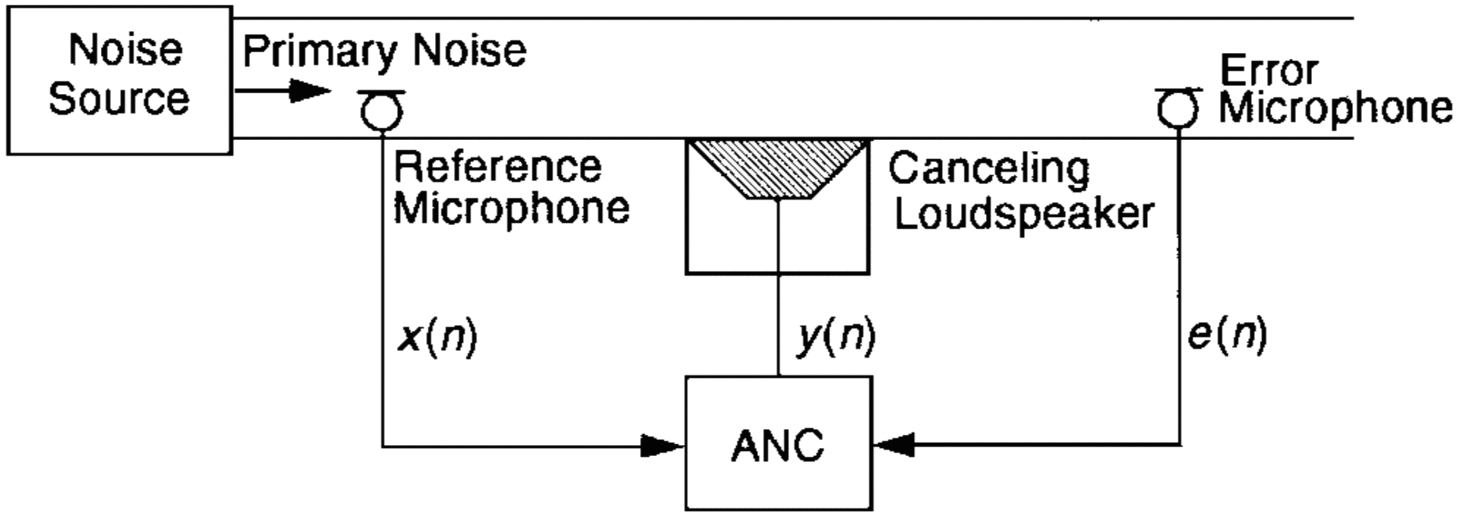
\includegraphics[height=0.2\textheight, width=0.7\textwidth]{images/kuo_ANC_gen_fdfw.png}
		\caption{Generic ANC Feedforward Block Diagram \cite{kuo}.}
		\label{fig:ANC_gen}
	\end{center}
\end{figure}

%% Other Solutions
\subsection{Other Solutions}

Other ANC methods can work purely in the time-domain. Since the signals are received and transmitted in the time-domain, frequency-domain transformation is not a necessary operation for functionality; frequency-domain transformation is just another option available when designing ANC. For example, the FXLMS ANC algorithm, which is discussed later with regards to the frequency-domain, can be implemented strictly in the time-domain \cite{kajikawa}.

ANC methods can also operate solely on feedback control, or utilize a hybrid system of feedback and feedforward control \cite{gaur}. Discussed later with feedforward control, the FXLMS ANC algorithm can also be designed with only feedback control \cite{roy}. In the case of feedback ANC, due to being affected by the generated anti-noise wave, the original noise wave is not directly accessible at the error microphone; thus, the original noise wave is instead approximated using the error signal and the output signal sent to the speaker \cite{roy}.

%% Performance Analysis
\subsection{Performance Analysis}

ANC performance can be experimentally tested using Fourier analysis. Spectral analysis can be used to determine the average frequency range in the region of concern \cite{chen}. DFT can be used on time-domain data to visualize the average noise power spectrum before and after the application of ANC. The pre-ANC and post-ANC average noise power spectra can be compared to establish the effectiveness of the ANC algorithm at nullifying targeted noise waves in the system. One method of comparing the two spectra is to subtract the post-ANC result from the pre-ANC result. The subsequent result of the subtraction is the residual average noise power spectrum after the application of ANC. Based on the residual average noise power spectrum, the ANC algorithm can be adjusted to further focus on frequencies where the power is significantly higher than the threshold (e.g. the threshold could be fixed at the mean of the residual average noise power spectrum).

\pagebreak

%% Filtered-x Least Mean Square Active Noise Cancellation
\section{Filtered-x Least Mean Square Active Noise Cancellation}
\label{sec:ANC_FXLMS}

A more advanced ANC algorithm uses the FXLMS adaptive filter, which is based on the Least Mean Square (LMS) adaptive filter \cite{kajikawa}.

%% Adaptive Filter
\subsection{Adaptive Filter}

An adaptive filter is a filter that iteratively updates its weights to adapt to recently observed data \cite{feintuch}. An example of an adaptive filter is LMS. Adaptive filters can be expressed in the frequency-domain.

The LMS adaptive filter computes the least mean square of the error (Fig. \ref{fig:LMS_fltr}). The time-domain LMS adaptive filter can be written as

\begin{gather}
    y(n) = \sum \limits_{k = 0}^{N - 1} b_k x(n - k) \text{ ,}\\
    b_k(n + 1) = b_k(n) + 2 \beta e(n) x(n - k) \text{ ,}\\
    e(n) = d(n) - y(n) \text{ ,}
\end{gather}

where $n$ is the sample iteration, $y(n)$ is the output of the adaptive filter at iteration $n$, $k$ is the index of the weight, $N$ is the total number of weights, $b_k(n)$ is the weight $k$ at iteration $n$, $\beta$ is the step size that determines convergence speed, $e(n)$ is the error signal at iteration $n$, $d(n)$ is the reference signal at iteration $n$, and $x(n - k)$ is the input signal at iteration $n - k$.

\begin{figure}[H]
	\begin{center}
		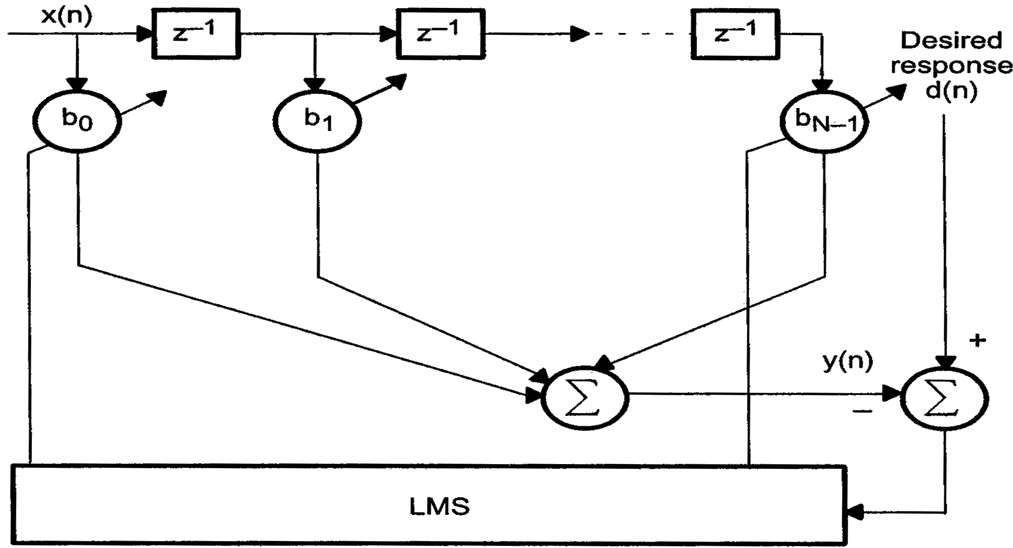
\includegraphics[height=0.35\textheight, width=0.7\textwidth]{images/roy_LMS_fltr.png}
		\caption{LMS Adaptive Filter Block Diagram \cite{roy}.}
		\label{fig:LMS_fltr}
	\end{center}
\end{figure}

\pagebreak

The frequency-domain LMS adaptive filter can be written as

\begin{gather} \label{eq:LMS_fltr}
    W_\omega(n+1) = W_\omega(n) + \mu \epsilon_\omega(n) X_\omega^*(n) \text{ ,}\\
    \epsilon_\omega(n) = D_\omega(n) - W_\omega(n) X_\omega(n)  \text{ ,}\\
    D_\omega(n) = P(j \omega) X_\omega(n) \text{ ,}
\end{gather}

where $\omega$ is the frequency bin, $n$ is the sample iteration, $W_\omega$ is the complex weight at $\omega$, $\mu$ is the step size that determines convergence speed, $\epsilon_\omega$ is the error signal at $\omega$, $D_\omega$ is the FFT of the reference signal at $\omega$, $P$ is the plant transfer function, $X_\omega$ is the FFT of the input signal at $\omega$, and $X_\omega^*$ is the complex conjugate of $X_\omega$ \cite{feintuch}.

%% Frequency-Domain, Adaptive Filter, and Feedforward Control Combination
\subsection{Frequency-Domain, Adaptive Filter, and Feedforward Control Combination}

The FXLMS adaptive filter is implemented similarly to the LMS adaptive filter. The application of the LMS adaptive filter in ANC results in an unsynchronized anti-noise wave due to the delay caused by the secondary path (defined later). A model of the secondary path is used to filter the input signal to account for the potential delay in the broadcasted anti-noise wave \cite{kuo}. As such, the input signal used in the LMS adaptive filter is replaced with a filtered input signal. $\epsilon_\omega$ in the LMS adaptive filter equation \ref{eq:LMS_fltr} is replaced with $E_\omega$. Then, in the context of ANC, the frequency-domain FXLMS adaptive filter can be represented as

\begin{gather}
    W_\omega(n+1) = W_\omega(n) + \mu E_\omega(n) X_\omega^*(n) \text{ ,}\\
    E_\omega(n) = H_M(j \omega) [P(j \omega) - H_S(j \omega) W_\omega(n)] X_\omega(n)  \text{ ,}
\end{gather}

where $\omega$ is the frequency bin, $n$ is the sample iteration, $W_\omega(n)$ is the complex weight at $\omega$ at iteration $n$, $\mu$ is the step size that determines convergence speed, $E_\omega(n)$ is the error signal at $\omega$ at iteration $n$, $H_M(j \omega)$ is the microphone transfer function, $P(j \omega)$ is the primary path transfer function, $H_S(j \omega)$ is the speaker transfer function, $X_\omega(n)$ is the FFT of the input signal at $\omega$ at iteration $n$, and $X_\omega^*(n)$ is the complex conjugate of $X_\omega(n)$ \cite{feintuch}. The context of these variables is given by the FXLMS ANC block diagram (Fig. \ref{fig:ANC_FXLMS}).

The block diagram in Fig. \ref{fig:ANC_FXLMS} shows how feedforward ANC incorporates an FXLMS adaptive filter to create the FXLMS ANC algorithm. The input signal $x(n)$ is the processed version of the noise source received at the reference microphone; the signal received at the reference microphone is sent through a hardware set that includes a pre-amplifier, anti-aliasing filter, and analog-to-digital converter \cite{kajikawa}. The primary path $P(z)$ is the channel from the reference microphone, or noise source, to the error microphone. The secondary path $S(z)$ refers to the set of signal processing operations done between the output of the FXLMS adaptive filter and the speaker, inclusive; this hardware set includes a digital-to-analog converter, reconstruction filter, power amplifier, region from the speaker to the error microphone, pre-amplifier, anti-aliasing filter, and analog-to-digital converter, in order \cite{kajikawa}. $\hat{S}(z)$ attempts to model the processes conducted on the secondary path. The $\hat{S}(z) \text{, FFT, IFFT, Complex LMS, and} W(z)$ blocks refer to the FXLMS adaptive filter as a whole. The summation junction of the output of the primary path and the output of the secondary path is representative of the error microphone \cite{kuo}; in other words, the superposition of the original noise wave and the broadcasted anti-noise wave is received by the error microphone. Finally, the error signal is transmitted as an input into the FXLMS adaptive filter.

 \begin{figure}[H]
 	\begin{center}
 		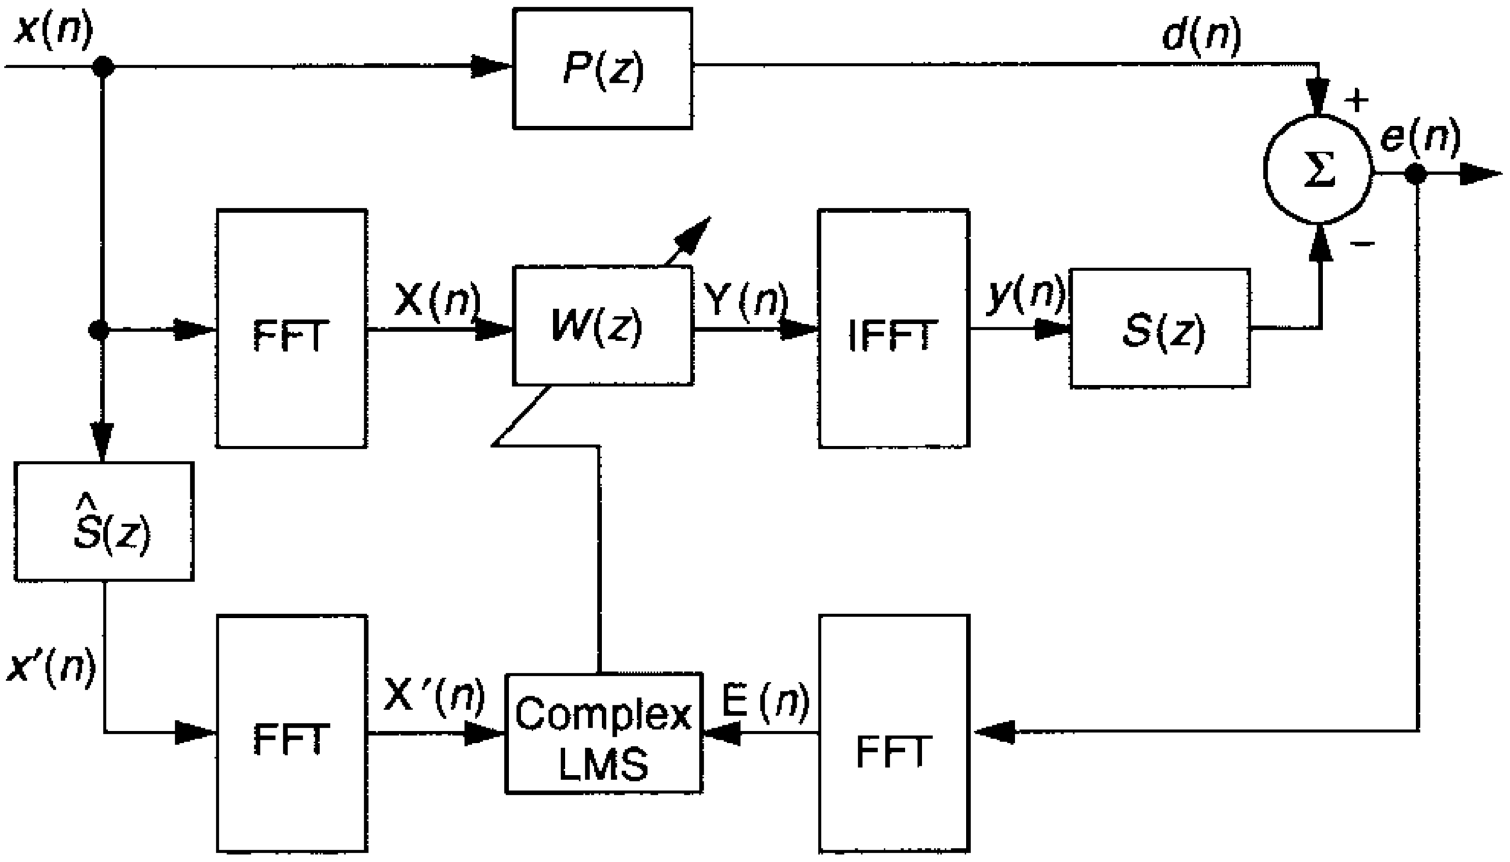
\includegraphics[height=0.3\textheight, width=0.7\textwidth]{images/kuo_ANC_FXLMS_fdfw.png}
 		\caption{ANC Feedforward Block Diagram using FXLMS Adaptive Filter \cite{kuo}.}
 		\label{fig:ANC_FXLMS}
 	\end{center}
 \end{figure}

%% Benefits and Drawbacks
\subsection{Benefits and Drawbacks}

One benefit of the frequency-domain approach to FXLMS ANC is that it reduces the total number of computations required for operation when compared with the time-domain approach to FXLMS ANC as a result of the replacement of convolutions calculations with multiplication calculations \cite{kuo}. A benefit of FXLMS ANC overall is that it incorporates an estimation of the secondary path, which enables the generation of a precise anti-noise wave \cite{gaur}.

One drawback of the FXLMS adaptive filter is that it converges slower than the original LMS adaptive filter \cite{gaur}. A couple of drawbacks of the frequency-domain FXLMS ANC algorithm are related to its practical implementation and use of computational resources. ANC devices such as headphones are small in size, and operate with limited computational speed and storage. The frequency-domain FXLMS ANC algorithm processes the input signal in batches to accommodate the necessary number of samples required for proper domain transformation \cite{kuo}; this may be important to note when defining an acceptable delay for real-time implementations. Also, in order to process the FFT of any given set of real-time data, it must be stored locally. The storage of frequency-domain data presents a trade-off between the granularity of the frequency bins and samples, and the amount of storage required. The nature of this trade-off for a single given signal can be captured as

 \begin{equation}
     d = N_f B N_s \text{ ,}
 \end{equation}

where $d$ is the total storage space required in bits, $N_f$ is the total number of frequency bins, $B$ is the size of each sample in bits, and $N_s$ is the total number of sample per frequency. For example, the upper range of human hearing is approximately $20,000$ Hz. If 64-bit floating-point values are used and the device stores one second worth of data, with an update rate of one millisecond, the total storage space required would amount to $20,000 \text{ bins} * \frac{64 \text{ bits}}{\text{sample}} * \frac{\frac{1 \text{ sample}}{0.001 \text{ second}}}{1 \text{ bin}} * 1 \text{ second} * \frac{1 \text{ megabyte}}{8,000,000 \text{ bits}} = 160 \text{ MB}$. The $160$ MB of storage required in this example is a significant amount of storage for a small embedded device, and substantiates the concern that a high granularity of frequencies and samples would require an unreasonable amount of storage.

%% Conclusion
\section{Conclusion}

This review provides a broad overview of acoustical noise cancellation: a brief discussion of PNC, detailed background of ANC, and an example of ANC in the frequency-domain using the FXLMS adaptive filter and feedforward control. ANC in technology is best known to the general public through acoustical noise cancellation used in noise-cancelling headphones; however, ANC may be more common in non-acoustic applications than in acoustical applications. Although the intricacies of network communications are not known to the general public, it is well-known that noise in RF applications is a significant consideration when designing the power of a transmitter or receiver. Thus, ANC can be used to improve the effectiveness of communications equipment \cite{darabi}. Further, ANC can be applied to electronic signals which can improve the performance of noise-intolerant components in the presence of extraneous noise \cite{teoh}. Overall, noise cancellation is a versatile technology which has been integral to the success of many projects in a wide range of fields.

\newpage

% References
\printbibliography[heading=bibintoc]

\end{document}